\chapter{Results and discussion}\label{ch:results}
%%%%%%%%%%%%%%%%
%- Introduction of what we are looking for, reminder of hypothesis
%%%%%%%%%%%%%%%%
This chapter explains the experimental data using the methods introduced in the previous chapter. For the X-ray pump-- X-ray probe study, data on heterogeneous clusters, i.e. helium droplets doped with xenon, have been taken at different time delays $\Delta t$. To complement the data, pristine data, i.e. helium droplets and xenon droplets individually, have been recorded at different time delays $\Delta t$ and the static case.\\
\begin{table}
	\centering
		\begin{tabular}{ | l | l | l | }
		\hline
			pump beam & probe beam & \  \\ \hline
			wavelength & 1.5 nm & 1.5 nm \\ \hline
			mean pulse energy & 1 & 1 \\ \hline
			pulse duration & 25 fs & 25 fs \\ \hline
			peak intensity in focus & 1 & 1 \\ \hline
			timing precision & 25 fs & 25 fs \\ \hline
		\end{tabular}
	\caption{caption TBD}
	\label{tab:caption}
\end{table}
MORE TEXT ABOUT EXPERIMENTAL PARAMETER TBD.\\
The chapter is organized as follows. Section \ref{sec:xenon-data} discusses the pristine xenon data and section \ref{sec:helium-data} covers the pristine helium data. Section \ref{sec:helium-xenon-data} shows the proof of principle that tampered layers mitigate radiation damage effects of an enclosed aerosol sample object.
%
%
%
%%%
\section{Pristine xenon pump--probe data}\label{sec:xenon-data}
%%%%%%%%%%%%%%%%%%%%%%%%%%%
%- Presentation of Xe data
%%%%%%%%%%%%%%%%%%%%%%%%%%%
\subsection{Xenon diffraction images}
%%%%%%%%%%%%%%%%%%%%%%%%%%%%%%
%- Present study of 1D condensed diffraction images.\\
%- Work out similarities to Tais radiation damage
%%%%%%%%%%%%%%%%%%%%%%%%%%%%%%
\begin{figure}
	\centering
		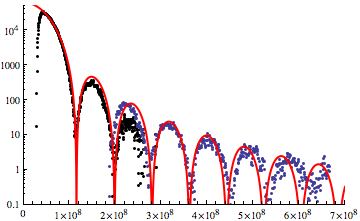
\includegraphics[width=0.49\textwidth]{images/results/Xe-only-0fs.png}
		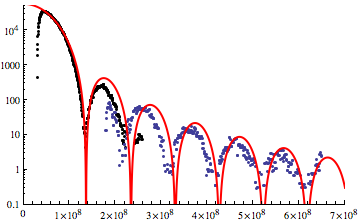
\includegraphics[width=0.49\textwidth]{images/results/Xe-only-60fs.png}\\
		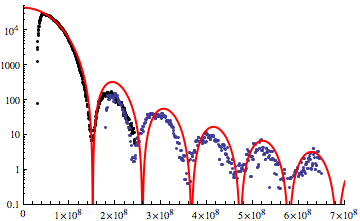
\includegraphics[width=0.49\textwidth]{images/results/Xe-only-120fs.png}
		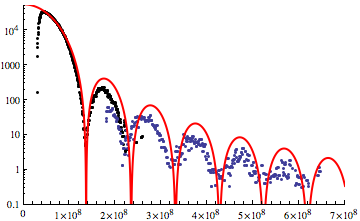
\includegraphics[width=0.49\textwidth]{images/results/Xe-only-250fs.png}\\
		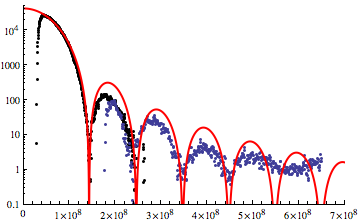
\includegraphics[width=0.49\textwidth]{images/results/Xe-only-400fs.png}
		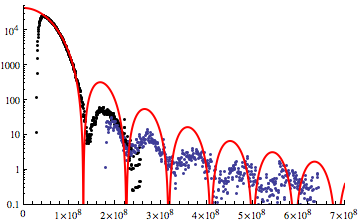
\includegraphics[width=0.49\textwidth]{images/results/Xe-only-800fs.png}
	\caption{caption}
	\label{fig:Xe-only-diff-pattern}
\end{figure}
Single xenon diffraction images have been selected using the hitfinder combination explained in section \ref{sec:hitfinding}. In brief, only hits that had high xenon charge states were selected. From this subset, another filter was applied that selected images with high signal on the pnCCD detector. Using these filters, a typical run of length 20 mins, i.e. $\sim 144,000$ images, was reduced to a subset of 30 - 60 images per run. These 30 - 60 images acceptable for reconstructions and it allows us the estimation that $0.02\% - 0.04\%$ of all imaged xenon cluster had good parameter for analysis. However, the hitrate in the live experiment was situated at $5\%-20\%$, which includes double or multi cluster hits and weakly scattering hits.\\
A 1D projection of selected diffraction pattern at time delays $\Delta t= \{0, 60, 120, 250, 400, 800\}$ fs can be found in figure \ref{fig:Xe-only-diff-pattern}. Per delay step $\Delta t$, the figure shows: A red line, which is the scattering as per equation \eqref{eq:scattering from sphere} fitted onto the low-$\vec{Q}$ signal of the zeroth diffraction scattering order. The black data points are projected from the rear pnCCD. The blue data points are projected from the front pnCCD. As the time delay $\Delta t$ between pump and probe pulse increases, the large-$\vec{Q}$ scattering signal decreases. This effect is similar to recent studies \citep{Gorkhover-2016-NatPho} performed on xenon cluster using an IR-pump and X-ray probe setup. It appears that the TBD\\
\begin{figure}
	\centering
		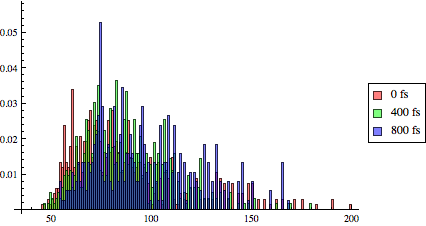
\includegraphics[width=1.00\textwidth]{images/size-distributions.png}
	\caption{caption. MAKE IMAGE NICER}
	\label{fig:size-distributions}
\end{figure}
The analysis of diffraction pattern also reveals a large scale characterization of the sample size. The size of several hundred single xenon cluster has been determined in figure \ref{fig:size-distributions}. Equation \eqref{eq:scattering from sphere} has be abused to semi-automate the size determination process, enabling high-throughput analytics. The size useful for a characterization of the source. The analysis shows that the size distribution follows a log-normal distribution PARAMETER. If the delay $\Delta t$ is increased, the mean of the log-normal distribution increases FROM TO. TBD
\begin{figure}
	\centering
		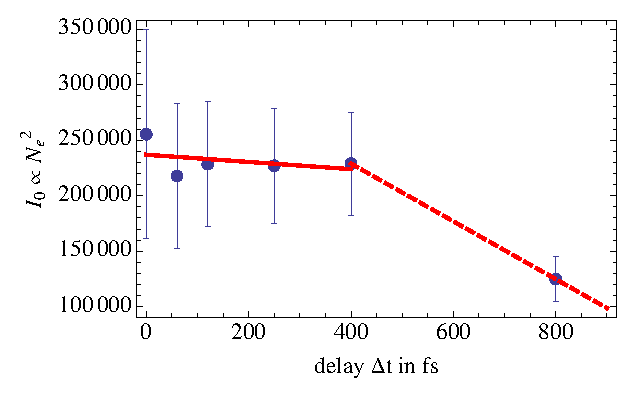
\includegraphics[width=1.00\textwidth]{images/results/number-of-scatterer.eps}
	\caption{caption}
	\label{fig:number-of-scatterer}
\end{figure}
The total number of scatterers, i.e. electrons that interact with LCLS, can be deducted from the diffraction patterns as well. As described in the theory section \ref{sec:saxs}, when
\begin{equation}
I\left(\vec{Q}\rightarrow 0\right)\propto N_{e}^{2},
\label{eq:}
\end{equation}
with the scattered intensity $I$ as a function of the scattering vector $\vec{Q}$ and number of electrons that contribute to the scattering process $N_{e}$. Figure \ref{fig:number-of-scatterer} shows the average fitting parameter $A$, which has been multiplied to equation \eqref{eq:scattering from sphere} to scale the intensity of the scattered curve, as a function of the time delay $\Delta t$ between the X-ray pump -- X-ray probe beam (blue dots) and several linear fits to simplify the interpretation (red lines). The averages were obtained in the analysis of about $\sim 15-30$ single xenon cluster diffraction pattern per delay step. The data show that the amount of electrons in the scattering system decreases only little. However, after a time delay of $\Delta t=400$ fs, the amount of scattering electrons decreases on average by $\sim 26 \%$. This could mean that the Coulomb trapping of the expanding nanoplasma is sufficient up to this delay step. At the delay step $\Delta t =800$ fs, the expansion of the cluster is in full process, thus the Coulomb potential decreases while the multistep ionization further energizes the system. Eventually, electrons overcome the Coulomb potential and dissipate the interaction region such that they do not contribute to the scattering anymore.
%
%
%
\subsection{Reconstructions of xenon cluster single shot images}
%%%%%%%%%%%%%%%%%%%%%%%%%%%%%%%%%%%%%%%%%
%- Present Xe - cluster reconstructions\\
%- Show 1D reconstructions and 'damage process'
%%%%%%%%%%%%%%%%%%%%%%%%%%%%%%%%%%%%%%%%%
\begin{figure}
	\centering
		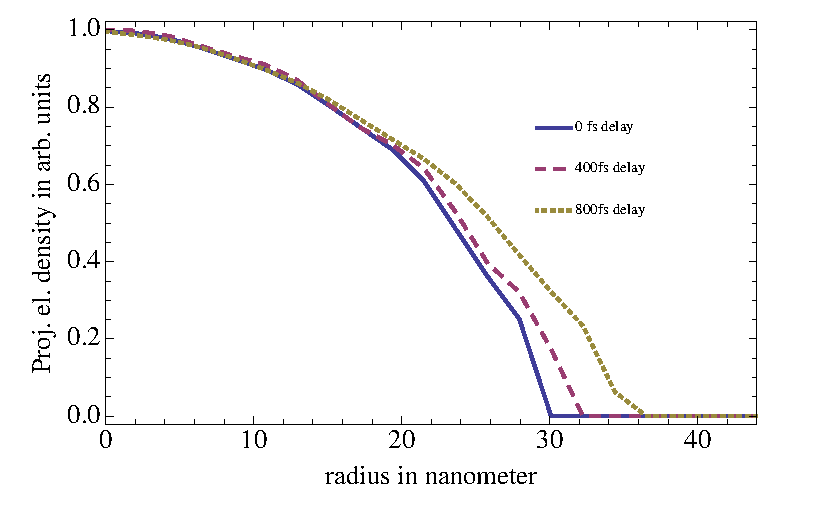
\includegraphics[width=1.00\textwidth]{images/results/Xe-reconstructions.eps}
	\caption{caption}
	\label{fig:Xe-reconstructions}
\end{figure}
1D reconstructions of single xenon cluster were obtained as described in section \ref{sec:1d-proj-and-phase-reconstruction}. Figure \ref{fig:Xe-reconstructions} shows 1D reconstructions of the projected electron density from single xenon cluster at time delays $\Delta t=\{0, 400, 800\}$ fs between the X-ray pump and X-ray probe beam. The density curves are normalized to clearly indicate an accelerated expansion of the outer atomic layers of the cluster. In this selection of hits, the cluster radii expand by $\sim 20\%$ over a time delay of $\Delta t=800 fs$, which is a substantial structural change. To make these events COMPARABLE INCLUDE DIFFRACTION PATTERNS. ELECTRON TEMPERATURE\\
For the sake of completeness, the recovered phase information and diffraction pattern are shown in FIGURE TBD.\\
%
\begin{figure}
	\centering
		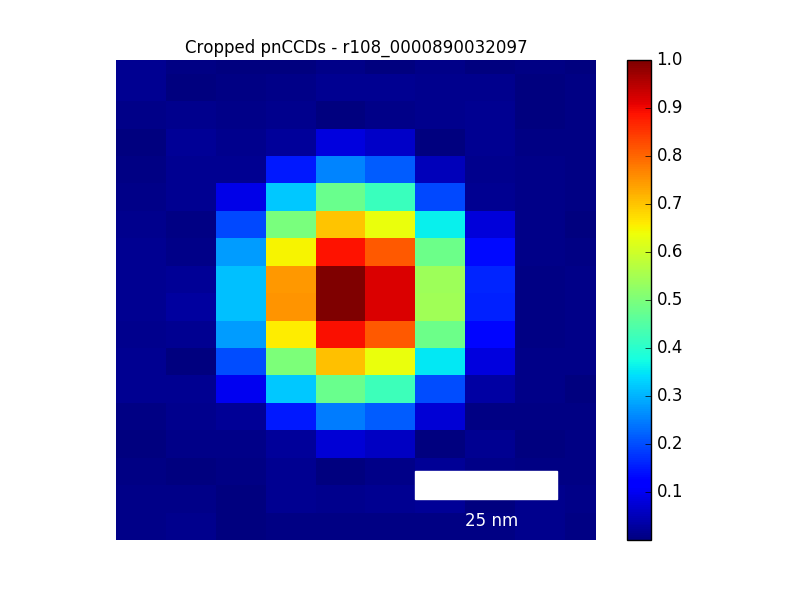
\includegraphics[width=0.49\textwidth]{images/results/Xe_0_fs.png}
		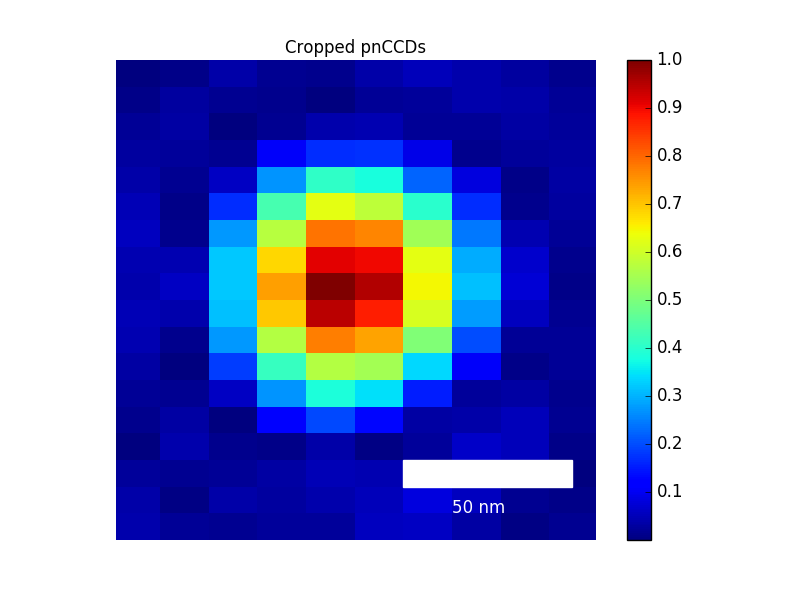
\includegraphics[width=0.49\textwidth]{images/results/Xe_800_fs.png}
	\caption{caption}
	\label{fig:Xe-2D-reconstructions}
\end{figure}
Figure \ref{fig:Xe-2D-reconstructions} shows 2D reconstructions of single xenon cluster at $\Delta t = 0$ fs (left) and $\Delta t=800$ fs (right). The cluster are appear generally spherical and of similar size. The signal-to-noise ratio is visibly better at $\Delta t=0$ fs than $\Delta t=800$ fs. This is due to the described loss of electrons, i.e. signal, in figure \ref{fig:number-of-scatterer}. Due to the normalization, the center of the projected electron density appears more dense, however, the loss of electrons in the center of the cluster flats out the overall density profile making the center of the normalized electron density appear more dense. The reconstruction at $\Delta t=800$ fs shows also a ringing around the actual cluster, which is likely an artifact of the spherical support structure and low signal-to-noise ratio and not an electron ring/hull around the cluster.
%
%
%
\subsection{Size-depended ionization pathways in atomic xenon and xenon clusters}
%%%%%%%%%%%%%%%%%%%%%%%%%%%%%%%%%%%%%%%%%
%- Xe iToF dynamics\\
%- Slightly more of Xe higher charge-states present at longer delays.
%%%%%%%%%%%%%%%%%%%%%%%%%%%%%%%%%%%%%%%%%
\begin{figure}
	\centering
		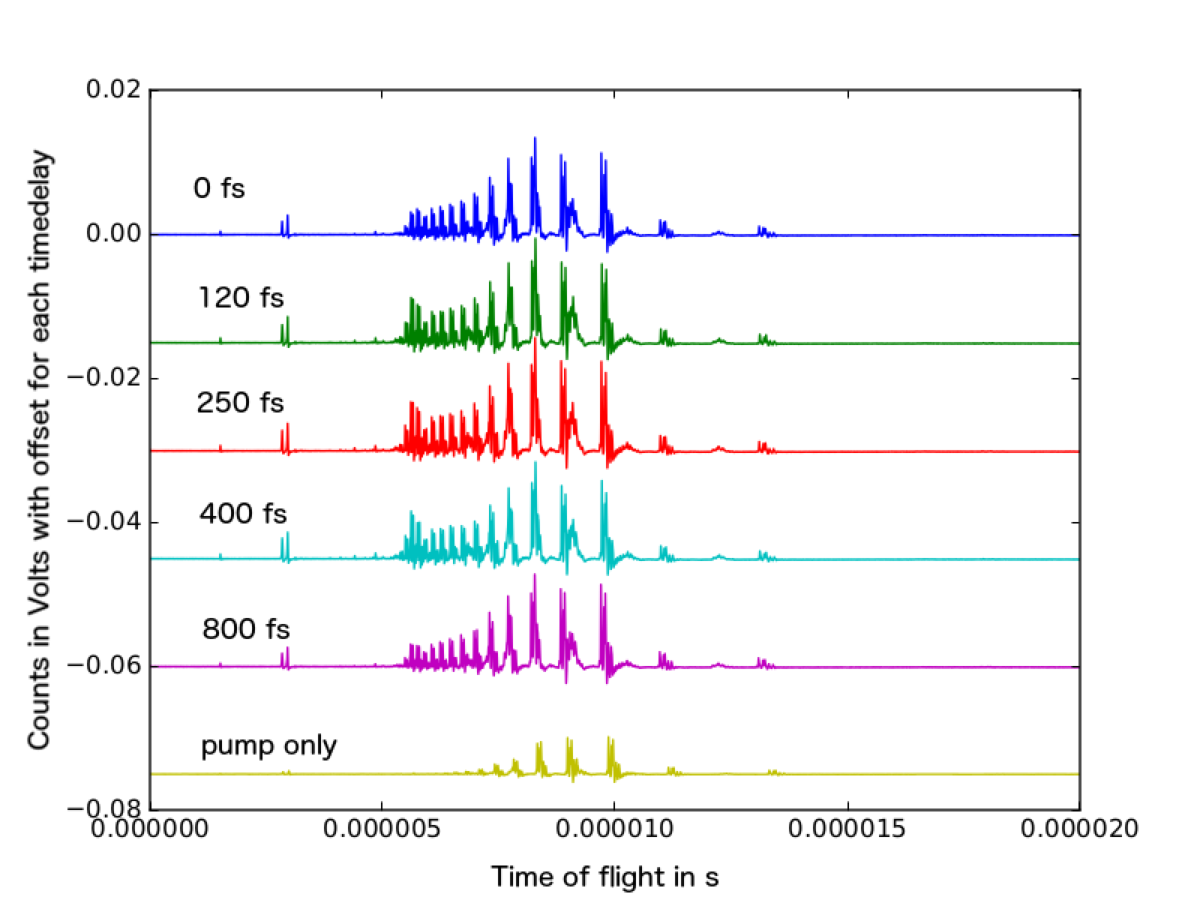
\includegraphics[width=1.00\textwidth]{images/results/TOF-atomic-xenon.png}
	\caption{caption}
	\label{fig:TOF-atomic-xenon}
\end{figure}
Ion time of flight traces of atomic xenon at different time delays $\Delta t = \{0, 120, 250, 400, 800\}$ fs and X-ray pump only data is shown in figure \ref{fig:TOF-atomic-xenon}. To create an atomic gas-jet, the experimental parameter at the source were changed to the reservoir pressure being $XXX$ bar and the timing was changed FROM TO. The time of flight data show a resonance type of behavior of the atomic xenon high charge states with a peak of high-charge state yield at $\Delta t = 250$ fs. The initial increase can be explained with a X-ray induced transparency increase (XITI) \citep{Schorb-2012-PRL} behavior of the atoms. The multistep ionization pathways after a time delay $\Delta t = 250$ fs appear less favorable for the creation of atomic high charge states.\\
\begin{figure}
	\centering
		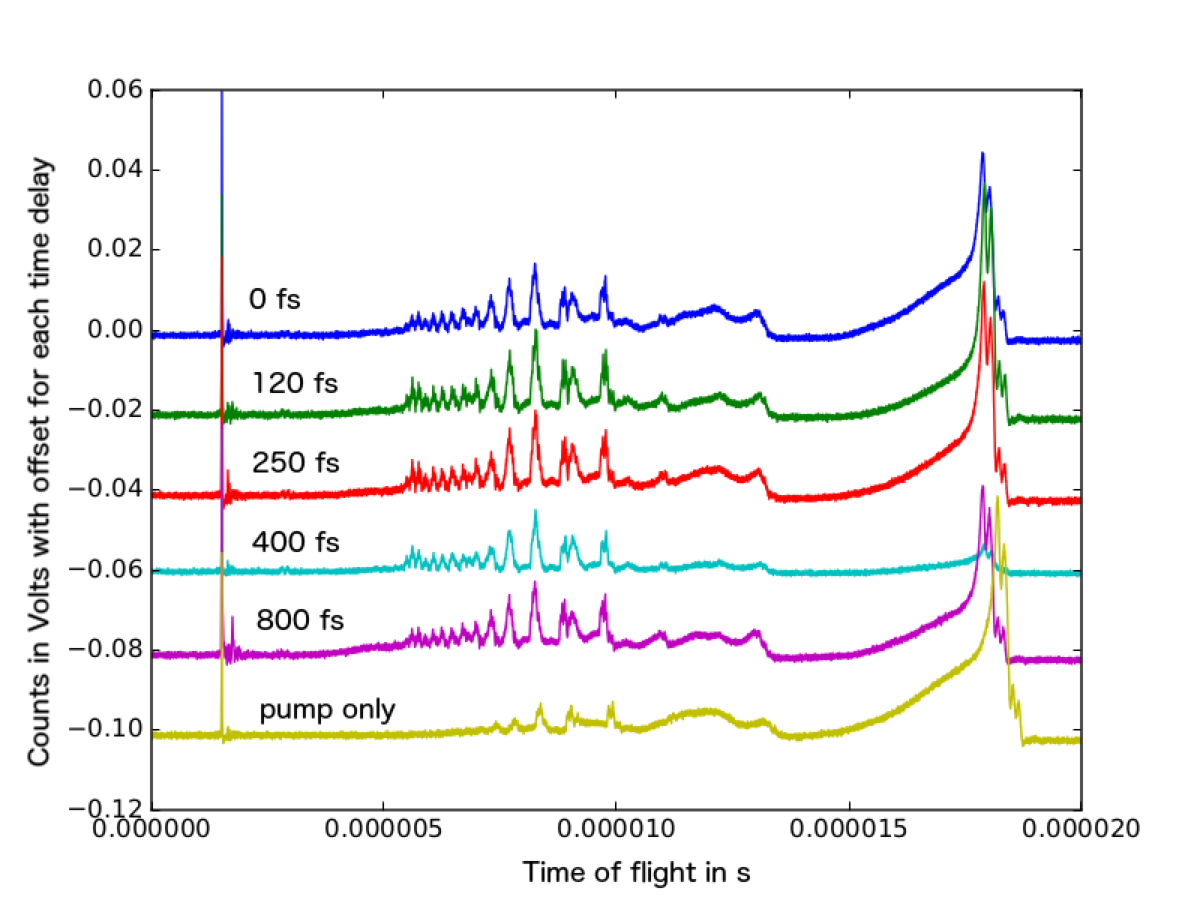
\includegraphics[width=1.00\textwidth]{images/results/TOF-small-cluster-xenon.png}
	\caption{caption}
	\label{fig:TOF-small-cluster-xenon}
\end{figure}
Figure \ref{fig:TOF-small-cluster-xenon} shows ion time of flight traces of small xenon cluster cluster at different time delays $\Delta t = \{0,120,250,400,800\}$ fs and X-ray pump only data. To create xenon cluster on the order of XXX nm radius the reservoir pressure in the source has been changed to $p_{0}=6$ bar. The data show similar resonant behavior as in the atomic case. Xenon high-charge states peak at a X-ray pump -- X-ray probe delay of 250 fs and start decrease at higher delays. At longer time of flight durations of 10 $\mu$s and beyond the small cluster signal dominates. Due to the short run times, the fluctuations of the cluster source vary the cluster signal significant.\\
\begin{figure}
	\centering
		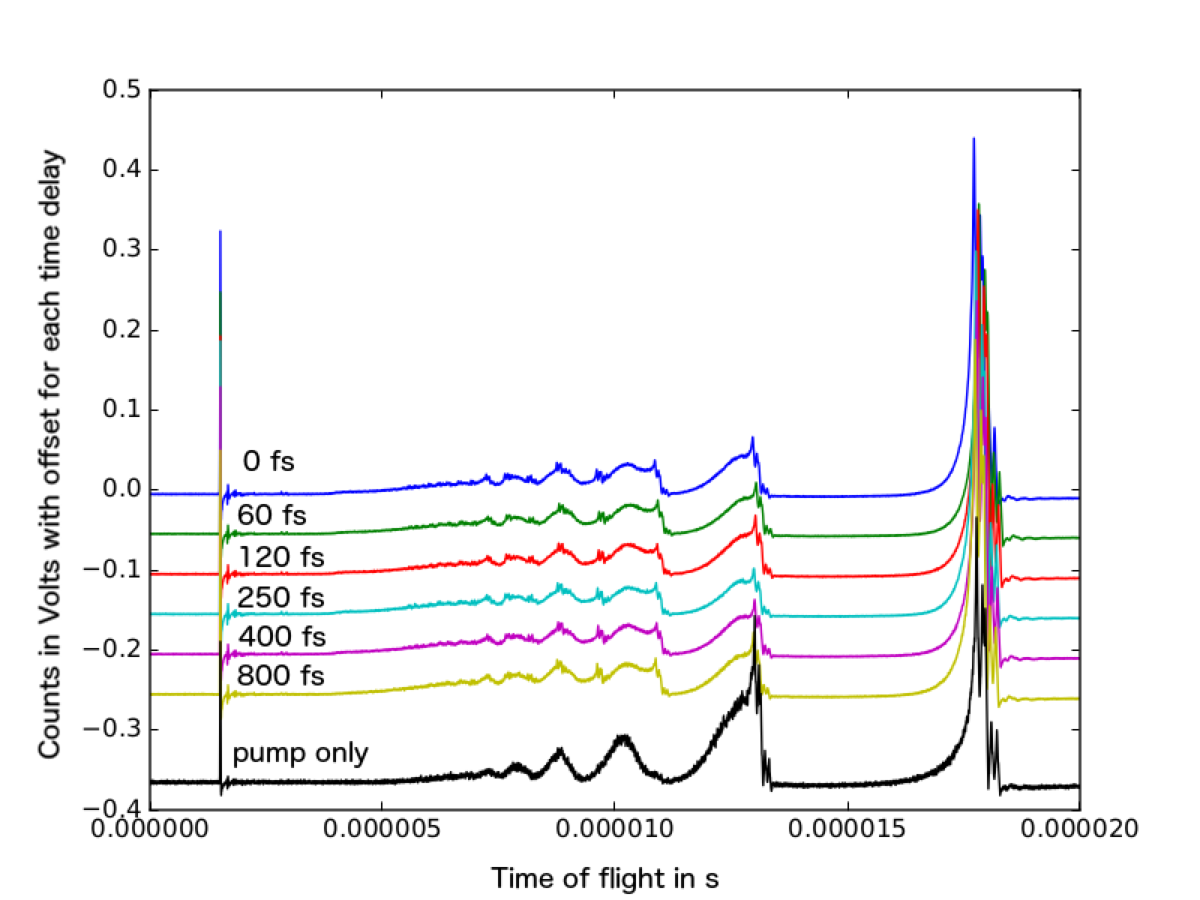
\includegraphics[width=1.00\textwidth]{images/results/TOF-regular-cluster-xenon.png}
	\caption{caption}
	\label{fig:TOF-regular-cluster-xenon}
\end{figure}
Ion time of flight traces of larger clusters can be found in figure \ref{fig:TOF-regular-cluster-xenon}. Here the source reservoir pressure has been adjusted to $p_{0}=20$ bar such that a mean cluster radius of XXX nm can be observed. The time delay between X-ray pump and X-ray probe has been set to $\Delta t=\{0,60,120,250,400,800\}$ and also the pump only data is shown. The data show that the cluster type of signal is dominating the trace. At a time delay $\Delta t=800$ fs, the xenon high-charge states increase, while no other dynamic appears obvious from the average data. The larger cluster ensemble may undergo a similar resonant type behavior as atomic xenon, however, the large cluster ensemble seem to affect the ionization pathways and thus the timescale of the resonant type behavior.\\
Summarizing, atomic xenon, xenon cluster of avgerage radius XXX nm and xenon cluster of average radius XXX nm were investigated using a X-ray pump -- X-ray probe setup and coincident spectroscopy and coherent diffractive imaging techniques. The ion spectroscopy data of Atomic xenon high charge states show a resonant type behavior as the time delay $\Delta t$ is varied from 0 fs to 800 fs. The resonance peaks around 250 fs. Small xenon cluster exhibit a similar behavior as atomic signal because atomic signal is dominating the high-charge states. The signal from larger xenon cluster of radii XXX nm is dominated by xenon charge fragments. An increase in the xenon high-charge states is observed at 800 fs, allowing us to conclude that the ionization dynamics have changed. It is interesting to note that altough larger cluster absorb overall more energy, the ensemble of atoms that is bound in the cluster is able to collectively change, here slow, ionization pathways. This behavior may be reproduced in other nano-samples such as bio-molecules or artifical tamper layers.
%
%
%
%%%%%%%%%%%%%%%%%%%%%%%%%%%%%%%%%%%%%%%%
\section{Spectroscopy on pristine and with xenon doped helium cluster}
%%%%%%%%%%%%%%%%%%%%%%%%%%%%%
% - Subsection for iToF data, important to compare to HeXe data.
%%%%%%%%%%%%%%%%%%%%%%%%%%%%%
\begin{figure}
	\centering
		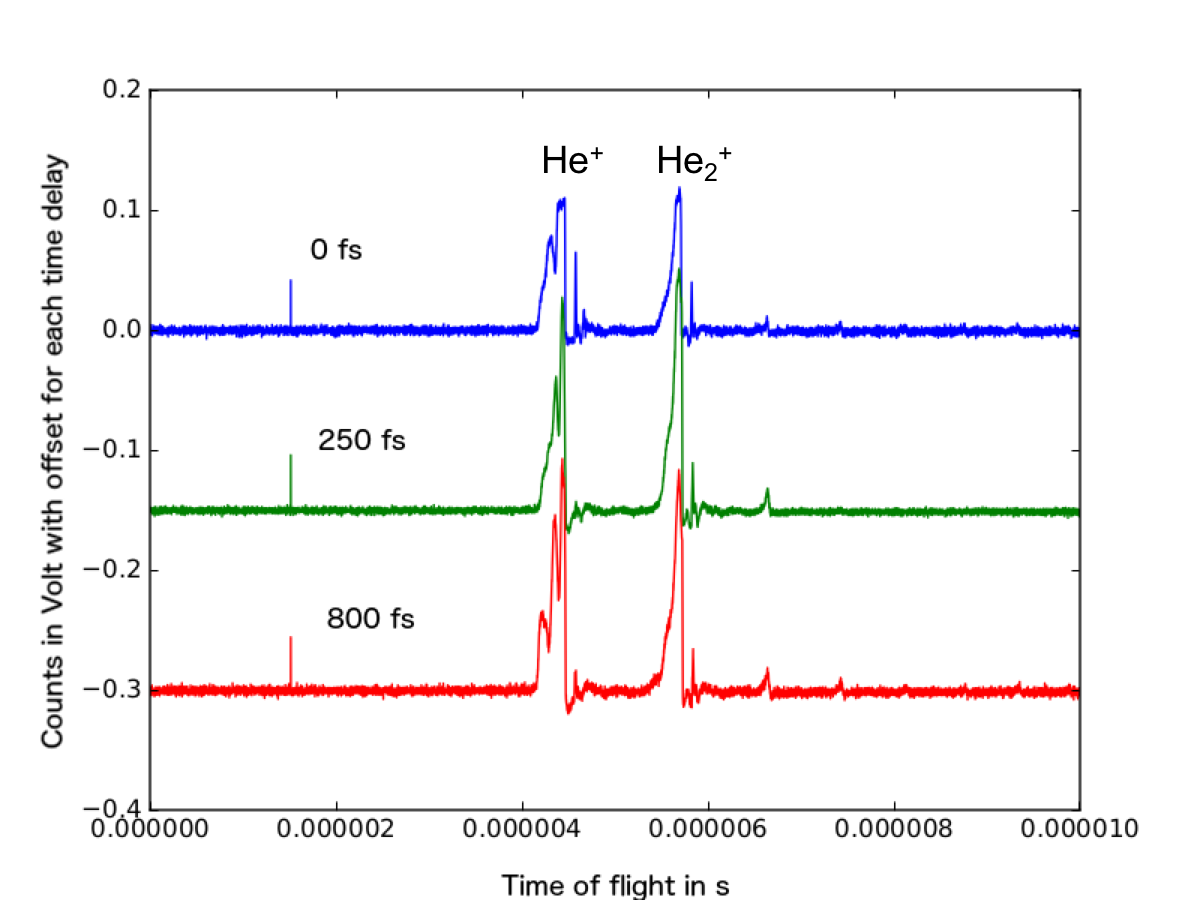
\includegraphics[width=1.00\textwidth]{images/results/TOF-helium-cluster.png}
	\caption{caption}
	\label{fig:TOF-helium-cluster}
\end{figure}
Figure \ref{fig:TOF-helium-cluster} shows the time of flight of pristine helium cluster charge fragments at pump--probe delays $\Delta t=\{0, 250, 800\}$ fs. The data show overall a similar behavior, regardless of the delay $\Delta t$. The traces indicate no contribution of doubly charged helium atoms. This can be explained to the comparably low absorption crossections of helium (see table \ref{tab:TBD}) and recombination rates TBD.\\
% \begin{figure}
% 	\centering
% 		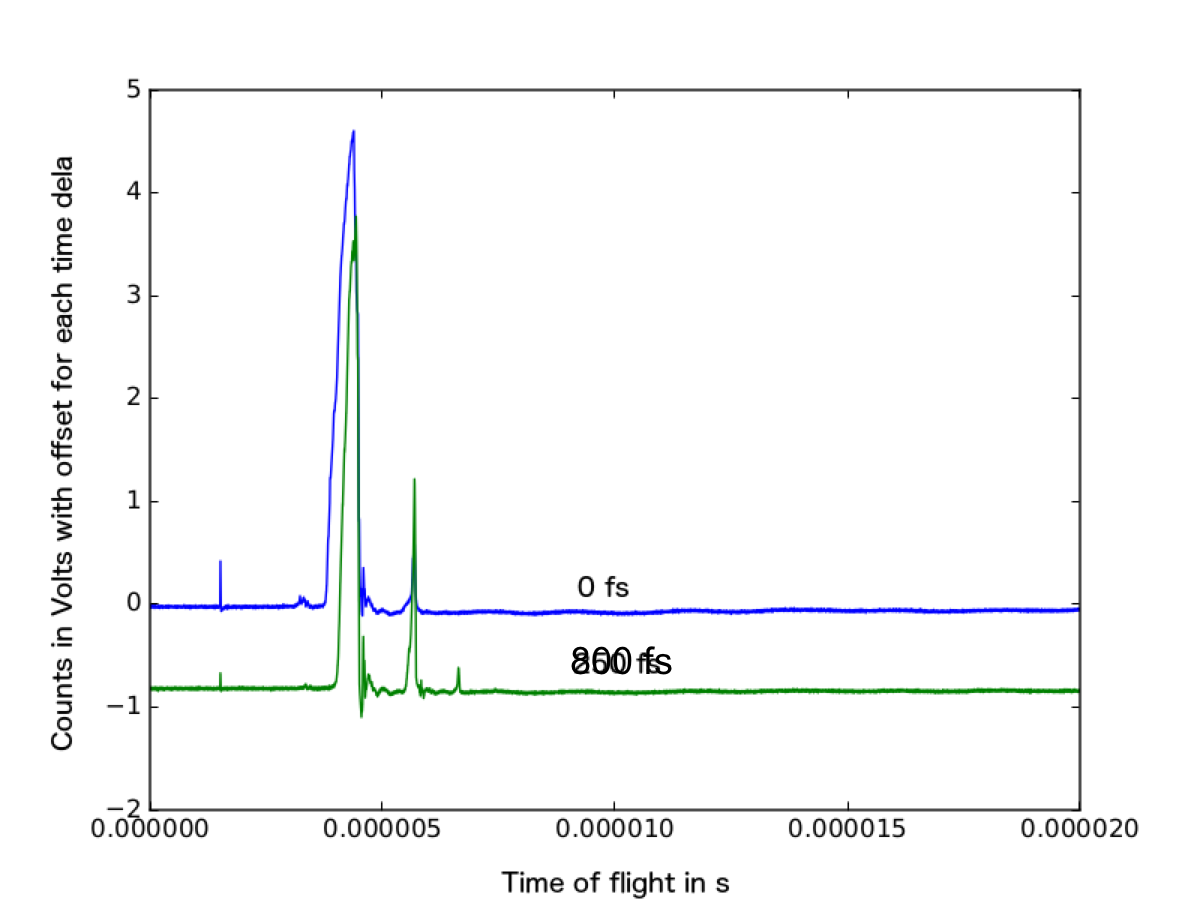
\includegraphics[width=1.00\textwidth]{images/results/TOF-helium-xenon-cluster-30.png}
% 	\caption{caption}
% 	\label{fig:TOF-helium-xenon-cluster-30}
% \end{figure}
% Figure \ref{fig:TOF-helium-xenon-cluster-30} shows flight times of with xenon LEVEL TBD doped helium cluster at pump--probe delays $\Delta t=\{0, 800\}$ fs. Most notably is now the presence of doubly charged helium $\text{He}_{2}^{2}$ and intense peak of the $\text{He}_^{+}$ ions. At different time delays $\Delta t$ the height of each peak shifts.The $\text{He}_{2}^{2+}$ states decrease in intensity but a stark increase in $\text{He}^{+}$ and $\text{He}_{2}^{+}$ states can be observed. However, no xenon charge states are present in the data with any significance.\\
\begin{figure}
	\centering{}
		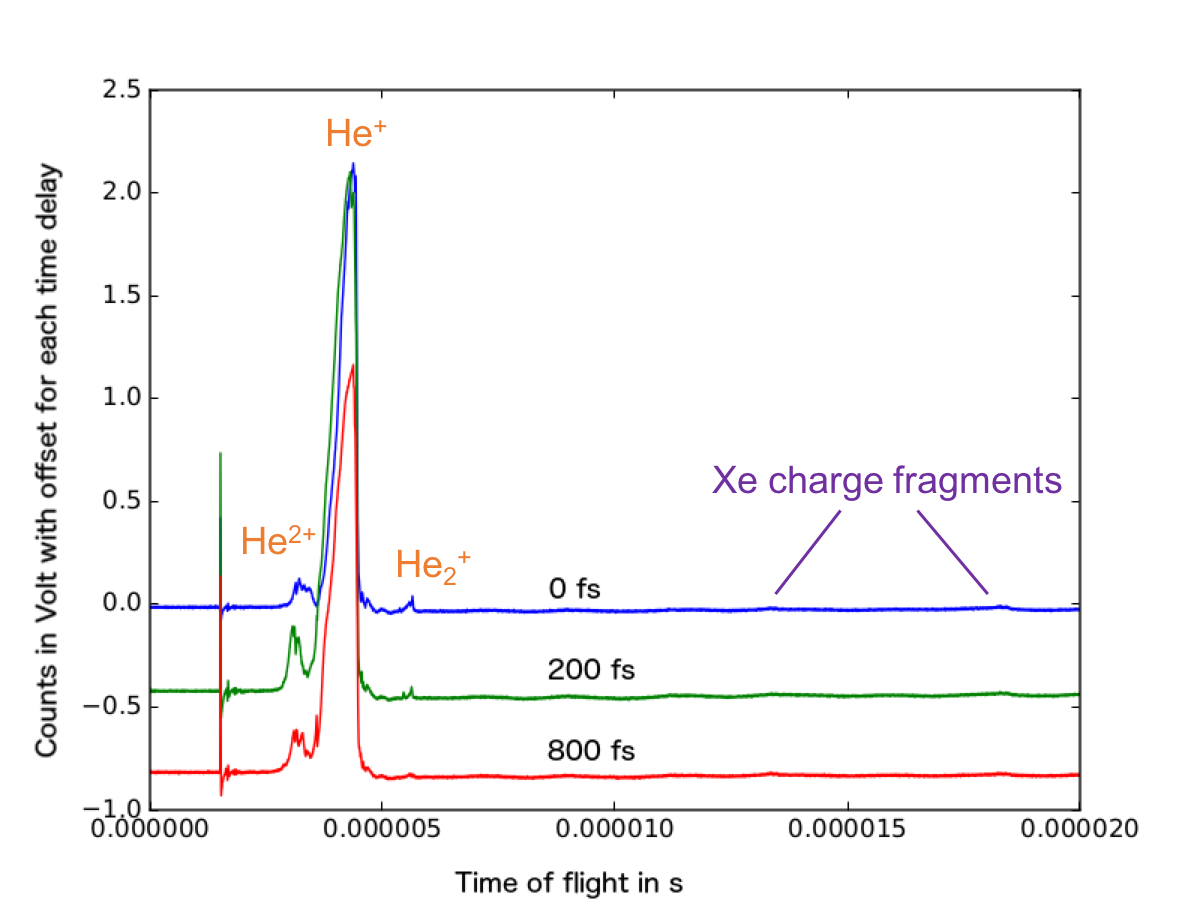
\includegraphics[width=1.00\textwidth]{images/results/TOF-helium-xenon-cluster-60.png}
	\caption{caption}
	\label{fig:TOF-helium-xenon-cluster-60}
\end{figure}
Strongly with xenon doped helium cluster time of flight traces are shown in figure \ref{fig:TOF-helium-xenon-cluster-60}. Most notably is that the data show a presence of the $\text{He}^{2+}$ state and strongly increased signal from $\text{He}^{+}$. Xenon charge fragments can be observed in at $\Delta t = 0$ fs. As the time delay $\Delta t$ is varied, the signal shows a distinct behaviour. A resonance type behavior is observed at $\Delta t = 200$ fs as the signal from $\text{He}^{2+}$ and $\text{He}^{+}$ peaks but is less intense at $\Delta t = 0$ and 800 fs. Conversly, the xenon signal and the helium dimer signal steadily reduces CHECK TBD.\\
Comparing the data from figure \ref{fig:TOF-helium-cluster} and \ref{fig:TOF-helium-xenon-cluster-60} allows us to conclude that xenon cluster transfer energy to the helium cluster that they are embedded in. This process is very efficient since the resonant behavior that origins from the xenon atoms is constituted in the helium signal, while the xenon signal steadily decreases. Therefore, the helium atoms function as electron reservoir and transport kinetic energy away from xenon atoms. This behavior is similar to \citep{TBD}. 
%
%
%
\section{Analysis of dynamics in diffraction images of heterogeneous helium-xenon cluster from X-ray pump--X-ray probe study}\label{sec:helium-data}
%%%%%%%%%%%%%%%%%%%%
% - Presentation of He data
%%%%%%%%%%%%%%%%%%%%%%%%%%

%
%
%
% \subsection{Diffraction images of helium cluster}
%%%%%%%%%%%%%%%%%%%%%%%%%%%%%%%%%%%%%%%
%- Work out radiation damage in 1D diffraction images.\\
%- Introduce envelope to show the radiation damage effect - important to compare to HeXe data.\\
%- Eventually subsection for reconstructions.
%%%%%%%%%%%%%%%%%%%%%%%%%%%%%%%%%%%%%%%
%
%
%
\section{Helium-xenon core-shell systems and pump--probe data}\label{sec:helium-xenon-data}
%%%%%%%%%%%%%%%%%%%%%%%%%%%%%%%%%%%%%%
%-Presentation of HeXe data
%%%%%%%%%%%%%%%%%%%%%%%%%%%%%%%%%%%%%%
%
%
%
\subsection{Time-of-flight data of helium-xenon core-shell systems}
%%%%%%%%%%%%%%%%%%%%%%%%%%%%%%%%%%%%%%%%%%%%%%%%%%%
%- Show dynamics of XeHe data in tof trace.\\
%- More hefty nanoplasma expansion in HeXe than in raw He.\\
%- Complement with simulations from Phay.
%%%%%%%%%%%%%%%%%%%%%%%%%%%%%%%%%%%%%%%%%%%%%%%%%%%
%
%
%
\subsection{Diffraction images of helium-xenon core shell systems}
%%%%%%%%%%%%%%%%%%%%%%%%%%%%%%%%%%%%%%%%%%%%%%%%%
%- Discuss diffraction images\\
%- Show how scattering intensity drops from He signal but not from Xe signal.\\
%- Eventually subsection for reconstructions.
%%%%%%%%%%%%%%%%%%%%%%%%%%%%%%%%%%%%%%%%%%%%%%%%%
%
%
%
\subsection{Core-shell system considerations}
%
%
%
\section{Static data}\label{sec:static}
%%%%%%%%%%%%%%%%%%%%%%%%%%%%%%%%%%%%%%%%%%
%-Include in other studies? Or appendix?
%%%%%%%%%%%%%%%%%%%%%%%%%%%%%%%%%%%%%%%%%%%%
%
%
%
\section{Conclusion of the X-ray pump -- X-ray probe study}
%%%%%%%%%%%%%%%%%%%%%%%%%%%%%%%%%%%%%%%%
%- Conclusion where the results are compared to each other\\
%- This experiment shows that heterogeneous clusters, as in tampered layers, do inhibit radiation damage of the sample target while the sacrificial layer undergoes a rapid nanoplasma transition.
%%%%%%%%%%%%%%%%%%%%%%%%%%%%%%%%%%%%%%%%%%
%
%
%